\label{organ}
%insert organization, schedule and cost estimates here

\subsection{Schedule}
The major milestones for the proposed CERN prototype detector construction and beam test is dictated by the DUNE overall schedule which foresees to place the first 10~kton detector module underground as early as calendar year 2021. Additional detector modules, possibly of different design, are expected to follow at intervals of 1-2 years in a technically driven schedule.
Information and results from the CERN beam test will inform decision on the DUNE far detector designs and hence should be available 
as soon as realistically possible. In addition, the LHC long shutdown, which is presently scheduled for mid-2018 represents a significant
constraint on the schedule.
In order to meet the requirements, cosmic muon data taking and ideally also beam data taking for the proposed measurement program 
should be complete prior to  the long LHC shutdown in mid-2018. 
Figure \ref{fig:schedule} shows a technically limited schedule which meets the above requirements.
%is based on experiences from the production and installation schedule for the 35~t detector.
This schedule is based on experience of designing and manufacturing components for the 35t detector which will be commissioned starting in July 2015 at  Fermilab.
\begin{figure}[h]
  \centering
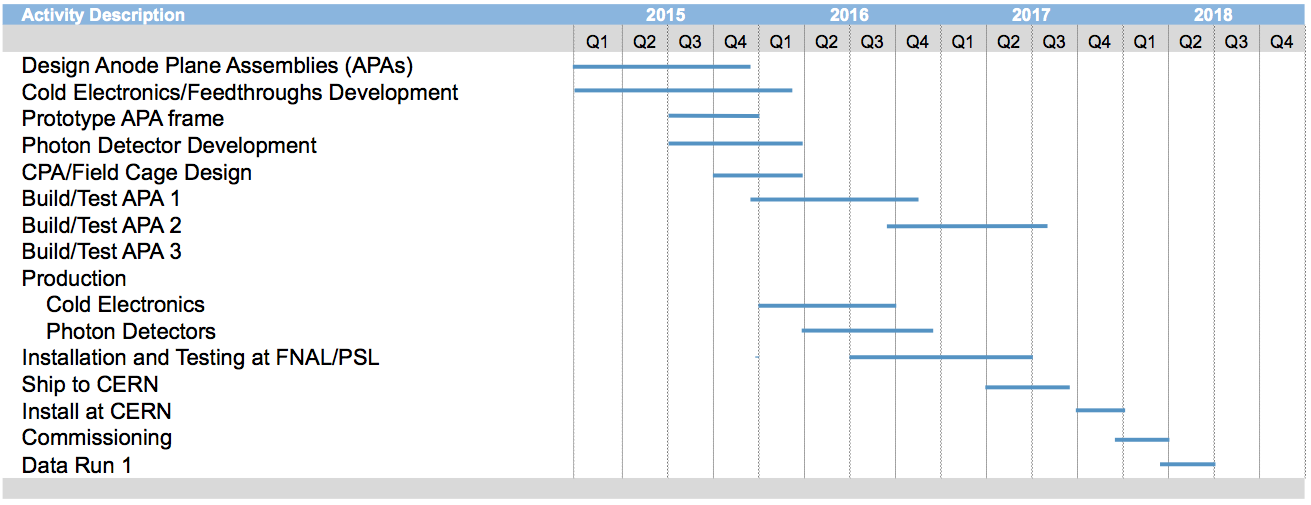
\includegraphics[scale=0.34]{figures/150219_schedule_3APAmod.png}
  \caption{THIS SCHEDULE NEEDS TO BE UPDATED WITH LATEST VERSION!!! Rolled up version of a draft schedule for manufacturing, installing and commissioning the CERN prototype detector. A 2 - 3 months data taking period is included in the schedule. }
  \label{fig:schedule}
\end{figure}


\subsection{Organization}

The CERN prototype effort is coordinated by the "CERN Prototype Technical Coordinator (CTC)" \cite{LBNEorg}.
The charge of the CERN prototype Collaboration Technical Coordinator is defined as follows.

The CERN prototype CTC is responsible for the following:
\begin{enumerate}[i]
	\item Prioritize and maintain a schedule of collaboration activities regarding simulations and physics analysis. 
	\item Prioritize and maintain a schedule of other collaboration service activities on the CERN prototype.  These activities may include collaboration participation in assembly, commissioning, calibration, debugging, data-taking, shifts, etc. 
	\item The responsibility of the CERN prototype CTC shall include maintaining a database of contributions from the collaboration to the CERN detector and beam test prototyping.
	\item The CERN prototype CTC shall recruit collaboration personnel and resources.
	\item The CERN prototype CTC shall coordinate with the DUNE far detector L-2 project manager and the DUNE technical coordinator
\end{enumerate}
There are currently two CTC sharing the responsibilities.

Several sub-groups are created to effectively execute the tasks required for the CERN prototype detector and beam test. These are: 

{\bf Measurement Program + Analysis}   Their charge is: to develop a comprehensive and prioritized list of measurements required to evaluate detector performance and provide detector charged particle response as input into DUNE physics sensitivity studies (beam physics, nucleon decay, supernovae, atmospheric neutrinos).  And to perform simulation studies to quantitatively compare the relevance of various measurements.

{\bf Beam} Their charge is: to work closely with the measurement group to identify ideal beam requirements, to work closely with the CERN beam group to develop realistic beam design to make relevant beam measurements, to evaluate and optimize possible beam injection points and beam orientations, to perform beam simulations and provide simulated beam spectra as input for detector response simulations, to identify required beam instrumentation for beam characterization, and to develop beam run plans.

{\bf Calibration}  Their charge is:  to develop tools to calibrate the performance of the detector, to interface with the physics measurement group to prioritize different calibration measurements, and to interface with detector subcomponent working groups to identify all required calibration tools and their integration into the detector /cryostat design.\\


The CERN prototype coordinators work closely with the DUNE far detector manager and the DUNE technical coordinator. 
Work on detector components is fully embedded in the DUNE project structure. The CTC also coordinates closely with the CERN Neutrino Platform
leader.\\
The leaders of the "measurement program analysis" subgroup work closely with the DUNE physics and software coordinators.
The leader of the "beam" subgroup works closely with the relevant CERN beam-line group leader.


\subsubsection{CERN single phase prototype personnel}

CERN prototype  Technical Coordinators (2014/15):\\
 Thomas Kutter (LSU) and Greg Pawloski (Minnesota)\\
 
 Measurement subgroup leader: \\
 \indent Donna Naples (Pittsburgh) and Jaroslaw Nowak (Lancaster)\\
 
 Beam subgroup leader: Cheng-Ju Lin (LBNL)\\

Calibration subgroup leader: \\
\indent  Qiuguang Liu (LANL) [interim] , Michele Weber (Bern)\\


\subsection{Division of Responsibilities}

Work on a MOU between the CERN nu-platform and DUNE describing responsibilities, listing institutions involved and defining deliverables is in progress. The following sections offer an overview of the current plans.

\subsubsection{Shared responsibilities}

The engineering design of the cryostat and the cryogenics system is considered to be a shared responsibility between DUNE/LBNF and CERN.

\subsubsection{DUNE responsibilities}

The following detector components are expected to be covered by the DUNE detector project:
\begin{enumerate}
\item XX APAs
\item CPA
\item field cage
\item cold electronics
\item DAQ hardware and software
\item ...
\end{enumerate}

The following items (incomplete list !) require further discussion. The responsibilities should be clearly spelled out.

\begin{itemize}

\item plans for data analysis and publications:\\
include: description of overlap/commonalities with WA105 data analysis and joined efforts

\end{itemize}




\subsubsection{CERN responsibilities}

\paragraph{The beam line:} design, setup of the beam line and beam monitoring instrumentation are expected to be provided by CERN.

\paragraph{The cryostat and cryogenics system:} are expected to be organized and paid for by the CERN nu-platform.
The scope of the EHN1 cryostat subsystem includes the design, procurement, fabrication, testing, delivery and oversight of a cryostat to contain the liquid argon and the TPC.\\
% moved here from chap 4 (by Anne)

\paragraph{DAQ requests:}  Data links of sufficient bandwidth to transfer the data files from the CENF to the CERN data center, and from there to locations worldwide for analysis. \\

\paragraph{Computing/Software support:} In order to leverage existing software and expertise, appropriate manpower will need to be allocated in order to create and maintain the computing infrastructure necessary for effective use of the reconstruction and physics analysis tools.\\



